\section{Design}
In order to make the application easy to use, design considerations have come from various existing map applications such as google maps and apple maps. These systems have heavily impacted the UI design of the application, so it can be familiar to user's coming from those platforms, making the system easy to use.

The design of the system happened in several in stages which are detailed below.

\subimport{./userstories/}{userstories.tex}

\subsection{Architecture overview}
With the system being modular and containing several key parts that need to function appropriately together and architecture overview diagram has been generated to show how the system intends to work. This architecture overview is useful for understanding the base system that has been implemented. It can be seen there are 3 main sections

\begin{itemize}
	\item Web application
	\item Android Application
	\item Rest API
\end{itemize}

Each of these sections alone focus as one large "module" 

\subsection{Data Storage}
Before development and to save times it's important to consider any data that may be required on the REST API. Using an Object Relation Manager (ORM) for handling of data is important for large projects and scalability. As an ORM is independent of SQL so the SQL dialect can be changed in the future if ever needed. An ORM's job is to also create the basic table structure and other elements for you. Although an ORM is being used it's still important to know the data that's required and the final structure of the data. Below is several database design standard showing how the final data structure should look.
\\
Some diagrams go here
\\
As can be seen from the data structure it's reasonably straight forward but contains all of the data that's required to store basic map information. The generated data structure within GoLang can be viewed in \appendixtemp

I don't know an erd I guess and data dictionary, maybe some other database design things here too. discuss the choices as well.

\subsection{Sequence Diagrams}
\subsection{Web Application}

\subsection{Android application}

\subsection{UI Designs}
There exists a range of map applications already implemented including Google maps, Waze \& apple Maps. Each mapping application has a similar UI but they do vary slightly. \appendixtemp contains some screenshots of each of these applications. With large companies having the budget to design optimum and efficient UI's the final product of the mapping system will be a combination of these UI's. Below is the intended UI designs for the applications each of these designed where made on Figma. Each image is a seperate frame, smaller frames are overlays and it will be explained how they fit with other frames.

\subsubsection{Android Application}
Below is a range of designs for the android application for the large parts of functionality. These designs are more detailed than the web application due to there being less "layers" of UI. The main functionality required for the android app is the ability to select maps, search, move around and set points. The below designs cover all of those requirements 
\fbox{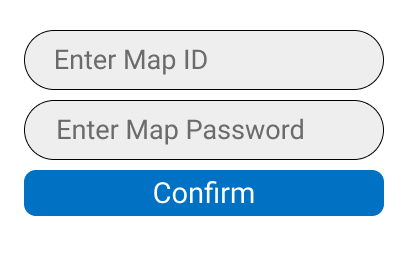
\includegraphics[height=6cm]{./images/designs/ui/android/AddMap.png}}
\fbox{\includegraphics[height=6cm]{./images/designs/ui/android/mapFilterOveralay.png}}
\fbox{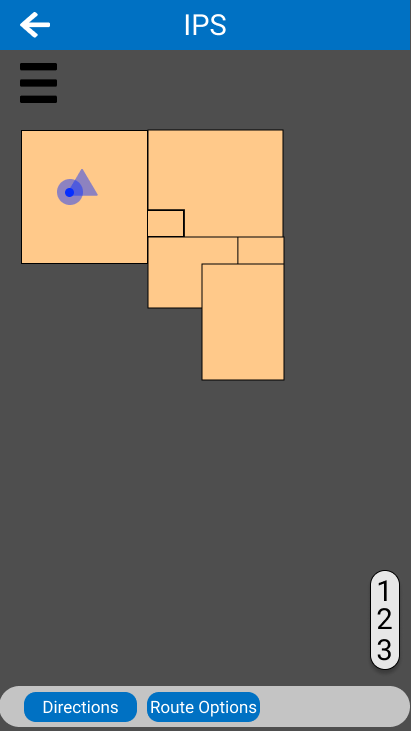
\includegraphics[height=6cm]{./images/designs/ui/android/Map.png}}
\fbox{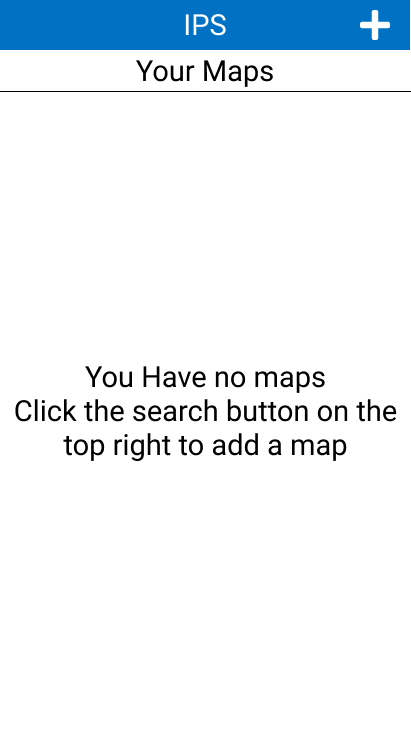
\includegraphics[height=6cm]{./images/designs/ui/android/MapSelection.png}}
\fbox{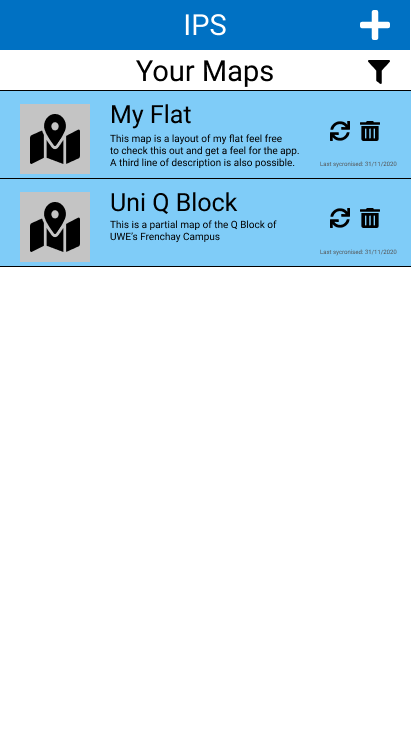
\includegraphics[height=6cm]{./images/designs/ui/android/MapSelectionWithmaps.png}}
\fbox{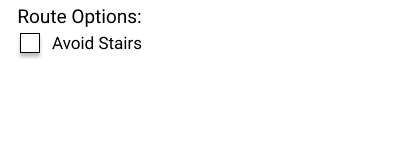
\includegraphics[height=6cm]{./images/designs/ui/android/RouteOptions.png}}
\fbox{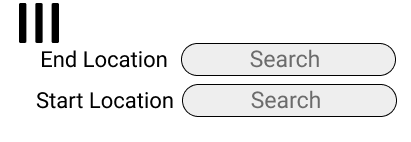
\includegraphics[height=6cm]{./images/designs/ui/android/RouteSearch.png}}
\subsubsection{Web Application}
